\documentclass[11pt,letterpaper]{article}																											  
\paperwidth=8.5in
\paperheight=11.0in
\usepackage[top=0.5in, bottom=0.5in, left=0.75in, right=0.75in]{geometry}
\usepackage{graphicx}
\setcounter{tocdepth}{2}
 
\begin{document}
	%\pagenumbering{gobble}
	\begin{center}
	\topskip0pt
	\vspace*{\fill}
	
\includegraphics[height=0.4\textheight]{logo} \\
	\linespread{2}
	\LARGE EECS Kinect Exhibit \\
	\Large Visualization Framework for Esoteric Sensory Devices \\
	\large Andrew DeMaria \\
	\linespread{1}
	\large Austin Diviness \\
	\large Aakash Shah \\
	\large Ryan Stauffer \\
	\large Matthew Stech \\
	\vspace*{\fill}
	\end{center}
	\pagebreak
 
	\tableofcontents
	%\pagebreak
	\newpage
 
	\pagestyle{plain}
	\setcounter{page}{1}
	\section{Introduction}
	\subsection{Client Description}
	The CSM EECS Department, represented by Professor Cyndi Rader and 
	Assistant Professor Yong Bakos, proposed and acted as contacts for this 
	project. During the fall of 2012, Professor Rader taught a course entitled 
	Readings in Software Engineering, where the class focused collectively to 
	write a project named Recycler Robbie. This project made use of the 
	Microsoft Kinect and OpenNI library in order to create a demonstration 
	game using hand tracking. The Kinect exhibit project evolved from the 
	results of this class.
 
	\subsection{Product Vision}
  After seeing the results of the Recycler Robbie project, Professors Rader and
  Bakos contracted the field session team to use the existing code base and
  create a standalone, open-source framework for multiple interactive
  visualizations. As this project is intended to live beyond the life cycle of
  the group, the framework would need to be designed such that future teams and
  students could easily adapt and contribute to the code base. These students
  would also be able to create and run their own visualizations utilizing the
  framework. 
	\pagebreak
 
	\section{Requirements}
	\subsection{Functional Requirements}
	\begin{itemize}
		\item Easy interfacing with additional visualizations created by students
		\begin{itemize}
			\item Programs can be inserted and made functional with minimal effort
			\item Support for Processing applets
		\end{itemize}
		\item Well-documented code base
		\begin{itemize}
			\item Original programs as examples
			\item Documentation explains the functionality and usage of SDK components
		\end{itemize}
		\item Facilitation of self-contained visualizations
		\begin{itemize}
			\item Modular and expandable
		\end{itemize}
		\item Use an easily accessible source revision control system for the code base
		\item Standalone, easily distributed, turn-key design
		\begin{itemize}
			\item Can be run without additional user input once started
			\item Can be easily configured for different user environments
		\end{itemize}
		\item Interactive exhibit using the Microsoft Kinect
	\end{itemize}

	\subsection{Non-Functional Requirements}
	\begin{itemize}
		\item Use Java with the Processing library
		\item Use the Colorado School of Mines Github as an easy, well known source revision control system
		\begin{itemize}
			\item Use Github's wiki capabilities to document the framework and facilitate student contributions
		\end{itemize}
		\item Ability to interface with additional input devices
		\item Legacy code refactored to meet the new goals of the project
		\item Transition between visualizations is coordinated by a launcher
	\end{itemize}
	\pagebreak

	\section{System Architecture}
	As the SDK is designed to be modular and expandable, it is capable of 
	communicating with both hardware devices via drivers, as well as graphical 
	libraries for displays. All of these libraries operate independently, 
	allowing a user to make use of whichever libraries they would prefer 
	without worry of conflicts. 

	For hardware devices, currently only the Microsoft Kinect is supported. 
	Data for the Kinect is gathered by interfacing with the OpenNI and Nite 
	libraries, and the provided data is processed and returned to modules that 
	use its information through the Input Services branch of the SDK. 

	For graphical libraries, the SDK supports multiple different graphical 
	programming methods. In addition to supporting Java's integrated AWT 
	rendering and console-based displays, the SDK also contains the core files 
	needed to use the Processing series of functions. Processing was initially 
	specified in the client requirements, and as such the team's primary focus 
	was put towards fully supporting Processing's library. All interaction 
	between these libraries is internalized within the SDK so users can use 
	the external libraries' functions without changing the design of their module. 
	(Figure 1)
	\pagebreak
   
	\section{Technical Design}

	\subsection{System Flow}

	At a high level, the system comprises of 3 primary subsystems: the modules,
	the Interface SDK, and the hardware. Modules are the user-developed units 
	that can be inserted into the system. The SDK as a whole provides both a 
	layer of abstraction and a platform for modules to run and communicate 
	with hardware devices. This is achieved by isolating the subsystems within 
	the SDK into module management, hardware management, and event management. 
	Module management is devoted to managing the lifecycle of modules and the 
	transitions between them. Hardware management pertains to abstracting away 
	details about the hardware by loading drivers. The Hardware Manager then 
	provides an interface for accessing these drivers. Event management 
	handles delegation of events to their registered receivers.

	Since the Module Manager controls the lifecycle of the program, a series 
	of initial steps must be followed in order for the framework to run. The 
	primary step is loading the Module Manager manifest file. The manifest 
	contains critical information such as the default module, the location to 
	load modules from, and the configuration store. The configuration store 
	maps arbitrary strings to configuration file locations, so as to be 
	accessed by any component that requires an external configuration file.

	Once the manifest is loaded, the Module Manager attempts to build a list 
	of all available modules. Availability is determined by the integrity of 
	the JAR, the availability of other required modules, and by checking requested
	hardware functionalities against the current hardware capabilities. Required
	modules and requested hardware functionalities are dictated by the module
	manifest which is located in each JAR. After this is completed, only available
	modules are remaining in the Module Manager's index of meta information on the
	modules. In addition, valid modules' meta-data is updated to reflect which jar
	the module can be found in.
	
	At this point, the Module Manager will allow the Hardware Manager to 
	initialize its assets. This includes loading its own Hardware Manager 
	manifest file, which includes information about all of the functionalities 
	and devices that the framework supports. Through this, the Module Manager 
	can give the Hardware Manager a module's hardware dependencies and receive
	feedback on if these dependencies are met. 

	Using this same process, the Module Manager can check whether the default
	module meets all its hardware dependencies. Checking its dependencies and
	indicating the default module in the Module Manager manifest is vital because
	the Module Manager relies heavily on the assumption that it can fall back to
	inflating the default in the case of a different module's failure. In the case
	where the default module fails, then the Module Manager will throw a fatal
	exception, which halts the framework's execution.

	Initially, the Module Manager loads the default module, and this is where 
	the main loop is entered and modules are loaded and executed. This 
	consists of a multitude of safeguards to ensure that the next module is 
	capable of running. First and foremost, the module manager attempts to inflate
	an instance of a Module. To do this, the Module Manager uses information in
	the Module manifest indicating which class to load, in which package this
	class can be found and the path of the JAR in which the module resides to
	instantiate an instance of a generic ModuleInterface.  A couple typical
	developer errors can occur at this point; first, the class may not be found
	because the reference to the class or package was invalid, or second, the
	class did not correctly extend from the current version for one of the
	abstract Module classes. Unfortunately, there are a few other less common
	errors that can occur at this stage including; the JAR file was tampered with
	after the Module Manager updated its index, or there was a breach in security
	policy for the class loader. However, if all goes well, the Module Manager is
	left with a proper instance of the ModuleInterface and it can continue.
	
	Next, is to check that the module's hardware dependencies are met. If so, the
	Hardware Manager attempts to build or re-build a cache of drivers, based on
	the next module's hardware requirements. Required functionalities have their
	drivers cached immediately at this step, while optional input types are cached
	at runtime when requested. In the case where any of these steps fail,  the
	Module Manager reverts to loading the default and repeats this process. It
	should be noted that the Module Manager will load the default module upon the
	current module's completion, unless directed otherwise.

	Once the setup process is completed, a semaphore is handed off to the running
	module so that it may signal the Module Manager for when it is finished
	executing. The design uses the Java provided CountdownLatch to implement this
	functionality. At this step, control is completely given to the running Module
	until terminated (TODO reference appendix for future work?).

	Once the running module terminates, control is returned to the Module Manager
	and the process of refreshing the internal list of modules is repeated. This
	is done in case JARs were added, removed or modified during the runtime of the
	previous module. Finally, the Module Manager repeats the full cycle of loading
	the next module as explained above.
	(Figure 2)

	\subsection{Modules}

	Modules are designed to be self-contained, flexible programs that can be 
	dynamically executed. To do this, modules are required to supply their own 
	manifest file indicating meta-information such as title, author, and icon, 
	as well as dependencies on both hardware and other modules. The manifest 
	provides the dependency information so that the Module Manager is able to 
	check whether the module is able to be executed.

	One key aspect about modules is that they are loaded independently of the 
	graphical library the modules use. This allows developers to use any 
	graphical library currently supported by the framework, such as Processing 
	or AWT.  This was accomplished through interfaces that abstract those 
	details away from the Module Manager.  This is also done through 
	delegation to a ModuleHelper, which helps facilitate communication with a 
	Module and the Module Manager. An example of data a module may request via 
	the ModuleHelper is the list of modules currently loaded or access to the 
	configuration file store.

	\subsection{Input Services}

	The hardware management subsystem is responsible for managing the physical 
	devices supported, their drivers, and the functionalities that they may 
	support. In order to abstract such detail away, a Hardware Manager 
	manifest is provided to help drive the design. The manifest consists of 
	several key pieces of information such as the functionalities and drivers 
	supported, as well as their classpaths.

	In order to abstract away the physical device from its capabilities, the 
	team split input services into two main components: functionalities and 
	drivers. Functionalities represent a form of data that can be generated by 
	a device, such as depth imaging. Drivers bridge the communication between 
	a piece of hardware and the functionalities it supports. In this manner, 
	an end developer only has to worry about the type of data they need, and 
	not the device that is producing it. However, the design does accommodate 
	for retrieving specific data from a specific driver, should it be desired. 
	Since functionality and driver information is loaded from the Hardware 
	Manager manifest, SDK contributors can also expand support for additional 
	devices with their own classes.

	Since a device can support multiple functionalities, a driver cache was 
	implemented to reduce overhead in reinitializing a driver. In between the 
	execution of modules, the driver cache is cleared and rebuilt from the 
	next module's requested input types. In order for a driver to be cached, a 
	series of validations are necessary. First and foremost, the functionality 
	supported by the driver must be required by the next module. For 
	optional functionalities, this check is performed at runtime. Second, a 
	given driver must adhere to the interface contracts for the 
	functionalities specified. Finally, an instantiated driver must indicate 
	whether it is available for use, a process specific to the device with 
	which the driver is communicating. If all of these prerequisites are met, 
	the driver is placed in the cache for the module's use. 

	During the runtime of a module, a developer may retrieve any driver 
	residing in the cache. To give developers as much control over their data 
	as possible, a driver list is provided for a given functionality. This 
	allows the developer to inflate any driver from the list. It's important 
	to note that since the driver cache is cleared in between module runtimes, 
	the developer does not need to be concerned about prior drivers' data 
	being persistent.

	While the developer should not have to be concerned about which device is 
	providing data, data from drivers can come in two forms. One is a 
	continuous stream of data, while the other is an event-driven system. The 
	continuous stream of data may be accessed whenever the developer wishes. 
	However, for the event-driven data, a developer must use the Event Manager 
	to retrieve data. Drivers automatically send their event information to 
	the event management system, and the developer must register receivers 
	that capture these events.
	(Figure 3)

	\pagebreak
   
	\section{Design and Implementation Decisions}

	During the development of this project, the team made several decisions that
	helped to shape the design of the framework. One of the first decisions was to
	continue using Maven as a software project management platform as used by the
	Readings in Software Engineering class. After initial exploration into the
	platform and the following learning curve, the team found Maven to be a
	flexible and adaptable tool for handling external libraries.

	The team wanted to let the end developers have the ability to configure the
	framework to meet their needs. This led to a configuration-driven design
	implemented using the XML specification. By using an XML design, the team
	enabled the developer to dynamically gather information about individual
	modules without having to modify the source code itself, increasing
	flexibility. 

	The idea of the Module was also introduced early in the development process.
	By creating a module archetype, the SDK could abstract away the graphical
	library the visualization wanted to use, if any. By doing this, the team was
	able to keep the Recycler Robbie game running, despite it using AWT for its
	graphical interface rather than Processing.

	Additionally, due to the decision to use an XML design, the team felt the need
	for modules to enforce a contract indicating its intents and characteristics
	before being loaded by the Module Manager. This was to ensure that a module's
	dependencies can be satisfied by the Hardware Manager and also be represented
	in a human-friendly manner. This led to the creation of the Module manifest
	for the modules that are loaded into the Module Manager.

	The Module Manager was necessary because the team wanted a way to manage a
	group of modules and the lifecycle of the exhibit. By having the Module
	Manager handle these aspects, the interaction between modules and their
	runtimes was greatly simplified. The Module Manager keeps track of several
	aspects of the exhibit, primarily the dependencies that modules require. This
	enables the manager to ensure that modules have an environment that satisfies
	these requirements. The Module Manager relies significantly on its
	communication with the Hardware Manager to verify these dependencies.

	The necessity to be able to swap out various devices led to the creation of
	the Input Services layer. Input Services needed to abstract away the physical
	devices and their drivers, so that modules can utilize the data they want
	without regard to which device is supplying that data. By having the Input
	Services abstract the specifics of a particular device driver into data
	interfaces, the polling of data by a Module can be standardized.

	Input Services has two separate entry paths.  Drivers can supply a continuous
	stream of data, or can be given at discrete intervals, such as depth imaging.
	Thus, the design needed to satisfy both methods of retrieval. For a continuous
	stream of data, modules are able to poll the driver at their leisure. However,
	for data given at specific times, an Event Manager had to be created to
	coordinate the propagation of data to receivers. The Event Manager's queuing
	system was designed to handle arbitrary data to aid expandability.

	The decision to centralize the receiving and reading of hardware data led to
	the creation of the Hardware Manager. The Hardware Manager was necessary to
	control access to the devices as well as provide information about the
	environment in which the modules run. An additional XML manifest file had to
	be loaded in order for the Hardware Manager to be configured with devices.

	The team was directed by the clients to use source control and chose to use
	Github for a central repository over other services. Github was selected
	because of the team's familiarity with the inner workings of Git, its
	friendliness towards open-source projects, and the preexistent Colorado School
	of Mines Github organization. Since one of the additional client requirements
	was to publish the framework as an open-source project, the team found Github
	to be an ideal distribution system that met this need.

	A further requirement set forth by the client was to have proper documentation
	and support for new developers to contribute to the SDK and develop their own
	modules. The decision to choose Github also addressed this requirement through
	the use of Github's wiki structure and integrated issue tracking.

	\pagebreak
   
	\section{Results}
	Our goal for this project was to create an open-source, interactive,
	visualization platform that can support user contributed visualizations, and be 
	demonstrated at any number of locations on campus. This was achieved by 
	creating an underlying architecture that would allow for a number of 
	arbitrary programs, referred to as modules, to be able to run on the system. 
	Modules can be created any number of ways, including the use of 
	Processing 1.5.1 as per the client requirements. The exhibit also 
	demonstrates the ability to catch the attention of passersby through eye-
	catching visualizations on the launcher.

	The modules, along with the other configuration driven aspects of the 
	framework, can also be deployed remotely such that physical access to the 
	hardware our project is hosted on is not necessary. Devices will still be 
	connected physically. Through this, we complete the requirement to provide 
	a turn-key based system. Our project does meet all the requirements 
	requested by the client. 

	The framework's code base has all been documented, both through the Github 
	Wiki and JavaDoc. The Github wiki also consists of setup \& installation, 
	tutorials, samples, and API documentation.

	Due to the complexity of the base architecture, the client requested that 
	we deprioritize refactoring the Recycler Robbie game in favor of 
	optimizing our design; because at that point, changes to recycler would 
	have been in the form of a port. That said, the game still performs under 
	our design. 

	Other aspects that could not be completed or tested due to time 
	constraints were support for Processing 2.0, OpenGL, and other sensory 
	devices (such as web cameras). In addition, there are no safeguards to prevent 
	inappropriate or malicious submissions. Neither the Twitter feed nor the 
	acmX game could be integrated into the system. The Twitter feed was purely 
	due to time constraints in that the information necessary to continue was 
	provided too late into our timeline. The completed acmX game relied on the
	aforementioned OpenGL and scene map data.  Although the scene map data is
	supported by OpenNI the team did not have this functionality integrated with
	the Input Services layer at the time.

	\pagebreak
   
	\section{Figures and Tables}
	\begin{figure}[h!]
		\caption{System Architecture}
		\centering
		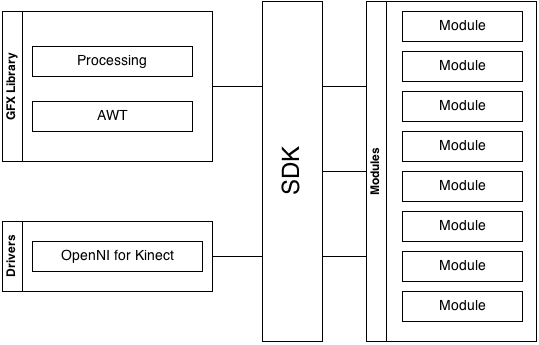
\includegraphics[width=0.9\textwidth]{overview}
	\end{figure}
	\pagebreak
	\begin{figure}[h!]
		\caption{System Flow}
		\centering
		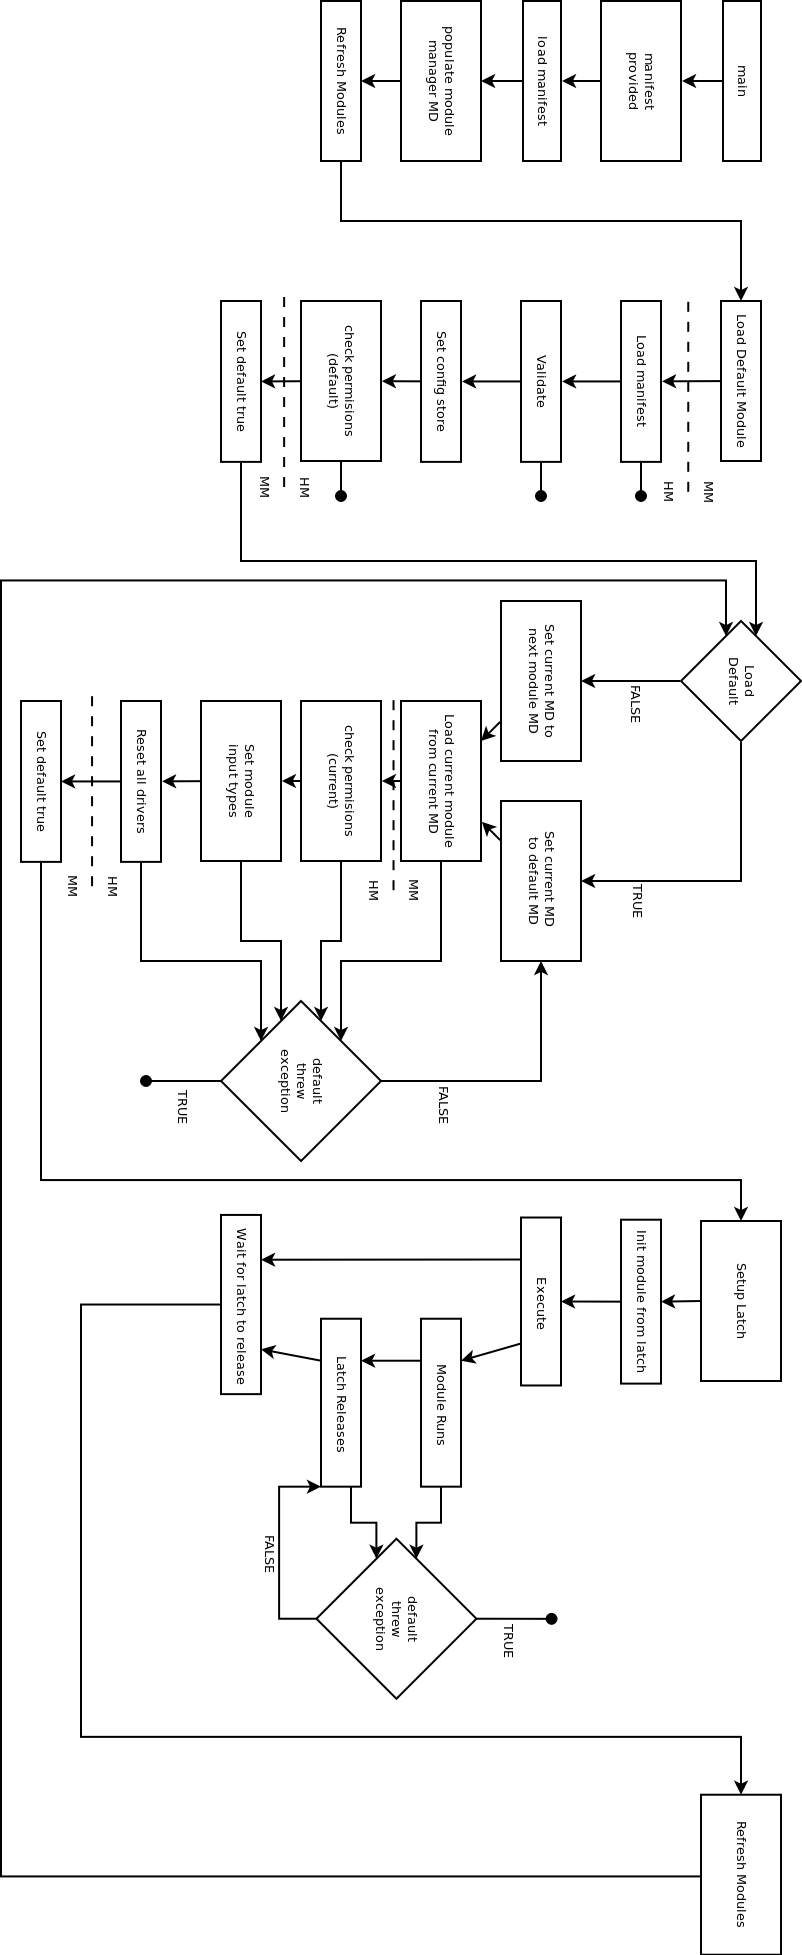
\includegraphics[height=0.9\textheight]{flow_diagram}
	\end{figure}
	\pagebreak
	\begin{figure}[h!]
		\caption{System Interaction}
		\centering
		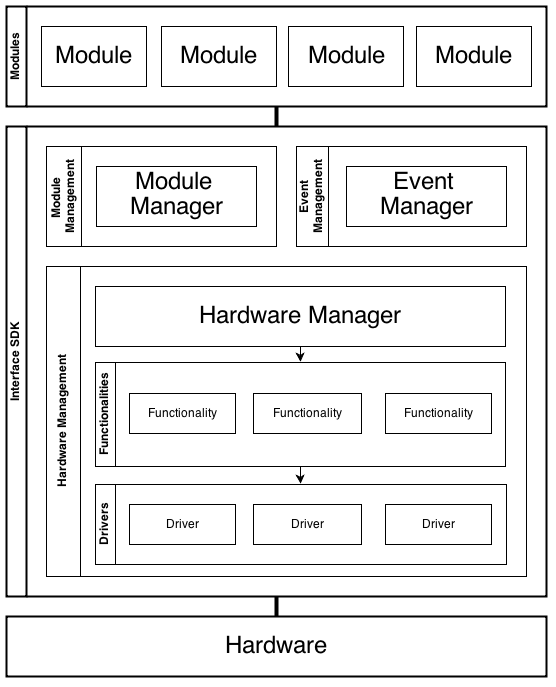
\includegraphics[width=0.9\textwidth]{interface_sdk}
	\end{figure}
 
 
\end{document}  
